%----------------------------------------------------------------------------------------
%	PACKAGES AND OTHER DOCUMENT CONFIGURATIONS
%----------------------------------------------------------------------------------------

\documentclass{article}

\usepackage{amsmath,amssymb,amsthm,latexsym,paralist,listings,graphicx}

\newcommand{\N}{\mathbb{N}}
\newcommand{\R}{\mathbb{R}}
\newcommand{\Q}{\mathbb{Q}}
\newcommand{\Z}{\mathbb{Z}}

\lstset{language=c}

%----------------------------------------------------------------------------------------
%	ASSIGNMENT INFORMATION
%----------------------------------------------------------------------------------------

\title{CSCE-452-500 Project\#1}

\author{Tropical Storm Ofo: \\ Beechner, Stella, Balli, DeGonge, Dobbs}

\date{9/27/2018}

%----------------------------------------------------------------------------------------

\begin{document}

\maketitle % Print the title

\section*{Project Summary}
Our team created a digital robot that can paint. Our robot has an arm with three joints and an end effector. Our software uses forward kinematics to determine the 2D coordinates of the end effector while the user paints by adjusting sliders related to the robots joints. There are many custimization options including: variable arm lengths, brush options, and customizeable colors.

\section*{Forward Kinematics}
For the forward kinematics, we store four 2D coordinates: three for the robot's joints, and one for the robot's end effector. Every time the user rotates an arm about its joint, the subsequent joints and end effector are also rotated about the same joint. The equations we use for rotation are equivalent to matrix rotation about the Z axis (i.e. the axis coming out of the screen). 

\begin{figure}
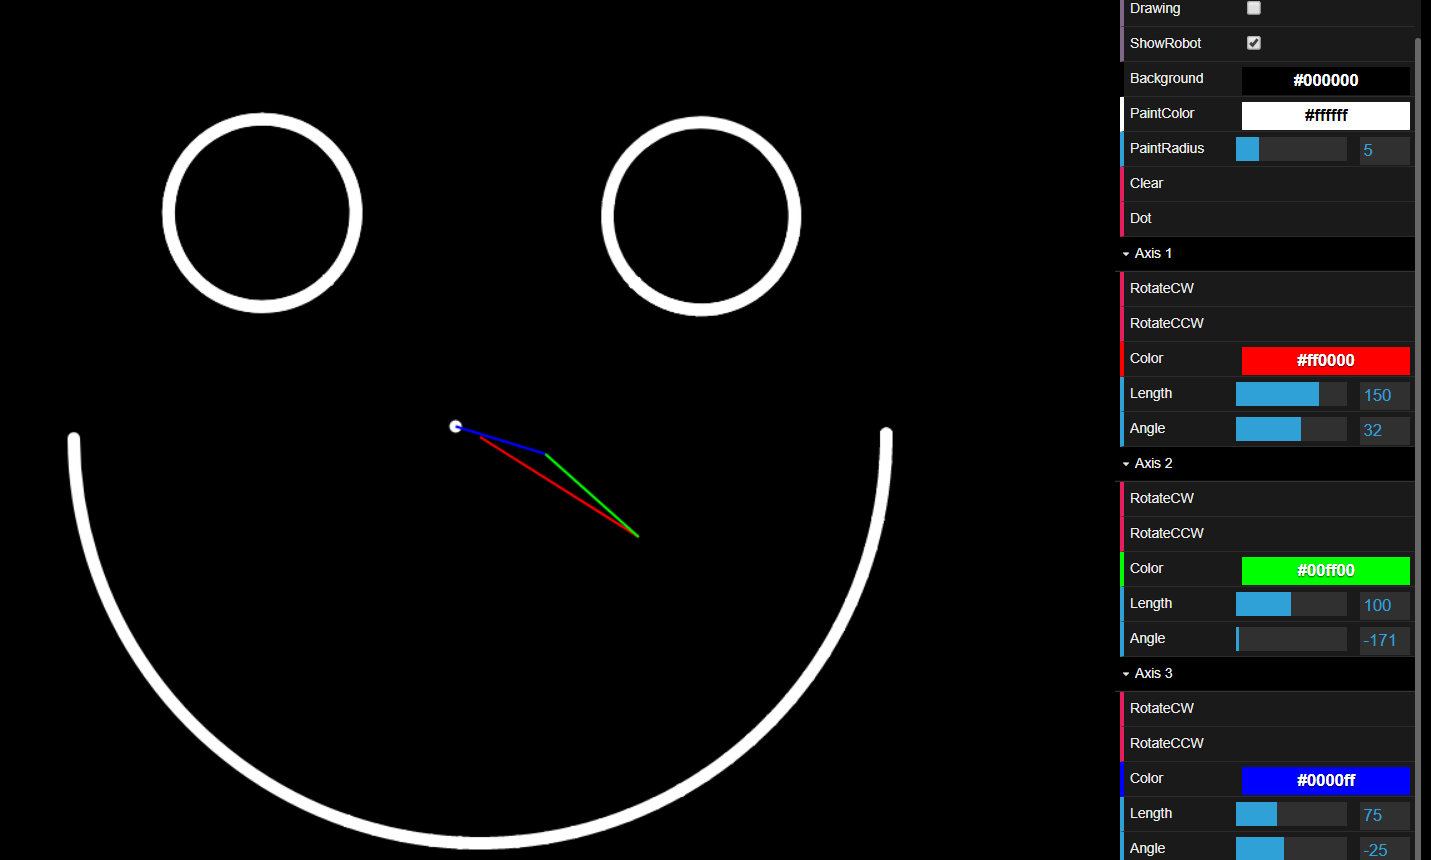
\includegraphics[width=\linewidth]{screen.png}
\caption{Screenshot of our robot}
\end{figure}

\end{document}
